\documentclass[11pt]{article}
\usepackage{amsmath}
\usepackage{graphicx}
\usepackage{multirow}
\usepackage{booktabs}
\usepackage{verbatim}
\usepackage{color}
\usepackage{hyperref}
\usepackage{url}
\usepackage{geometry}
\usepackage{esvect}
\usepackage{esdiff}
\usepackage{siunitx}
\usepackage{caption}
\usepackage{subfig}
\usepackage{gensymb}
%\textwidth 17cm
%\evensidemargin -0.5cm
%\oddsidemargin -0.5cm
\geometry{margin=2.5cm}
%\setlength{\belowcaptionskip}{-10pt}

\title{Ganymede PhiO Coordinate System}
\author{Isaac Wetton}
\date{\today}

\begin{document}
\maketitle

\noindent The GPhiO coordinate system is a fixed coordinate system which is defined by the corotation velocity vector at Ganymede (Phi, $\phi$) and the Jovian spin axis (Omega, $\Omega$) \cite{nasagan}. These vectors are perpendicular to one another. Phi is positive in the direction of corotation and Omega is positive northward.

Ganymede's $\phi$ is the X-coordinate whilst $\Omega$ is the Z-coordinate. The Y-coordinate completes the right-handed set and points towards Jupiter from Ganymede. Basis vectors of the system are fixed at the satellite's closest approach \cite{nasagan}.

\begin{figure}[!htb]
    \centering
    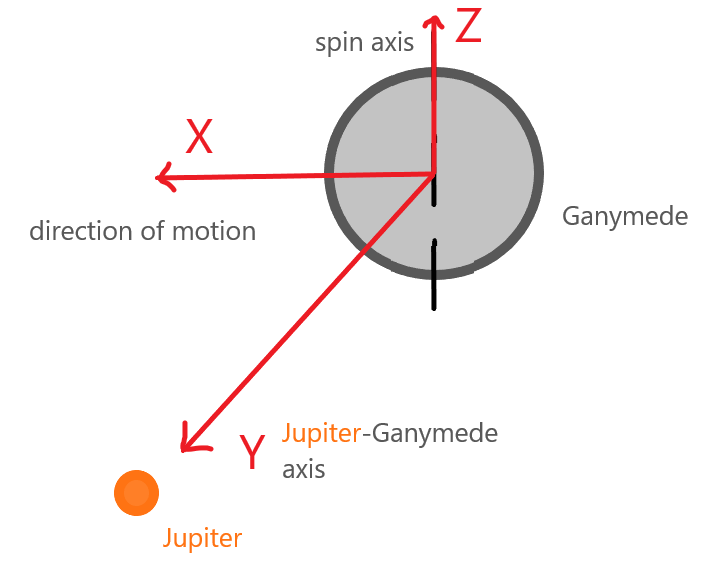
\includegraphics[width=12cm]{GPhiO.png}
    \captionsetup{width=13cm}
    \caption{A diagram illustrating the GPhiO coordinate system. It shows that X is in the direction of Ganymede's motion, Y is in the Ganymede-Jupiter axis, and Z is Ganymede's spin axis.}
    \label{fig:GPhiO}
\end{figure}

\noindent A visualisation of the coordinate system with respect to Jupiter can be seen in figure \ref{fig:GPhiO}. The X coordinate is in the direction of Ganymede's velocity, the Y coordinate is in the direction of Jupiter from Ganymede, and the Z coordinate is the spin axis, completing the right-handed set \cite{flybylines}.

\bibliographystyle{unsrt}
\bibliography{bibliography.bib}
\end{document}
